\documentclass[UTF8]{ctexart}
%\documentclass{article}
\usepackage{graphicx,amsfonts,amsmath,mathrsfs,amssymb,amsthm,url,color}
\usepackage{fancyhdr,indentfirst,bm,enumerate,natbib, float,tikz,graphicx}
\usepackage{caption}
\usepackage{subcaption}
\usepackage{calligra} % 添加书法字体包

\title{24实用随机过程期末}
\author{} % 改用书法体
\date{}

\textheight 23cm
\textwidth 16.5cm
\topmargin -1.2cm
\oddsidemargin 0cm
\evensidemargin 0cm

\begin{document}

\maketitle

\noindent 1.(每小题 6 分,总 30 分)设有一个质点在如图所示的二叉树上(共 $m=3$ 层)作随机游走:它从顶点 0 出发,每隔单位时间等概率沿边转移到某一个邻点上.以 $X_{n}$ 表示该质点经过 $n$ 步跳之后所在顶点的编号,则 $\left\{X_{n}, n \geq 0\right\}$ 为一个 Markov 链。\\
\begin{figure}[h!]
	\centering
	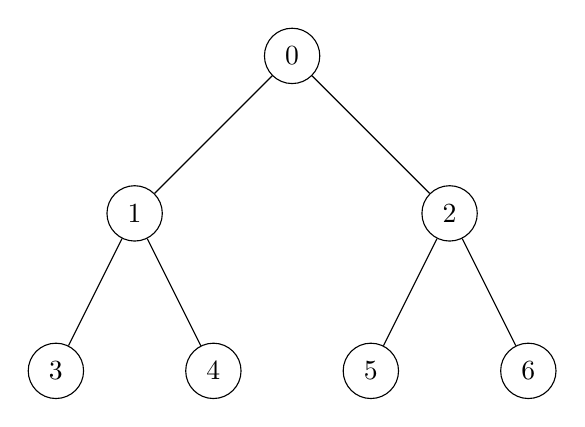
\begin{tikzpicture}
		\tikzset{
			box/.style ={
				circle, %圆形节点
				minimum width =20pt, %最小宽度
				minimum height =20pt, %最小高度
				inner sep=3pt, %文字和边框的距离
				draw=black, %边框颜色
				fill=white
			}
		}
		\node[box] (1) at(0,0){0};
		\node[box] (2) at(-2,-2){1};
		\node[box] (3) at(2,-2){2};
		\node[box] (4) at(-3,-4) {3};
		\node[box] (5) at(-1,-4){4};
		\node[box] (6) at(1,-4){5};
		\node[box] (7) at(3,-4){6};
		\draw[-] (1)--(2);
		\draw[-] (1)--(3);
		\draw[-] (2)--(4);
		\draw[-] (2)--(5);
		\draw[-] (3)--(6);
		\draw[-] (3)--(7);
	\end{tikzpicture}
\end{figure}

\noindent (1)试写出 $\left\{X_{n}, n \geq 0\right\}$ 的一步转移概率矩阵 $\bm{P}_3$ .\\
(2)对任意顶点 $k(0 \leq k \leq 6)$ ,讨论其周期性和常返性.\\
(3)对任意顶点 $k(0 \leq k \leq 6)$ ,求质点从 $k$ 出发后第一次返回到 $k$ 所需平均步数 $\mu_{k}$ .\\
(4)在稳态条件下,该 Markov 链是否都是时间可逆的?证明你的结论.\\
(5)对一般的 $m(m \geq 1)$ ,试求该 Markov 链的平稳分布.\\
解:(1)一步转移概率矩阵为
\[
\bm{P}_3=
\begin{pmatrix}
	0 & \frac{1}{2} &\frac{1}{2} & 0 &0 &0&0\\
	\frac{1}{3} & 0&0 & \frac{1}{3} &\frac{1}{3} &0&0\\
	\frac{1}{3} & 0&0 & 0 &0 &\frac{1}{3}&\frac{1}{3}\\
	0 & 1 &0 & 0 &0 &0&0\\
	0 & 1 &0 & 0 &0 &0&0\\
	0 & 0&1 & 0 &0 &0&0\\
	0 & 0&1 & 0 &0 &0&0\\
\end{pmatrix}
\]
(2)所有状态互通,对于每个状态至少需要两步回到自身,则所有的状态的周期为2\\
又Markov链是不可约有限状态的,则所有状态都是正常返的\\
(3)利用有限加权边图上的随机游走的结论,对存在的每条边赋权重$w_{ij}=1$,就满足上述转移概率矩阵,且有\\
\[
\sum\limits_{i,j}^{} w_{ij}=12
\]
上式是因为每条边(共6条)要计数两遍(这样比单独计数每个状态的边之后再相加来的方便)\\
\[
\pi_i=\frac{\sum\limits_{j}^{} w_{ij}}{\sum\limits_{i,j}^{} w_{ij}}
\]
\[
\pi_i=
\begin{cases}
	\frac{1}{6}  &  i=0 \\
	\frac{1}{4} &  i=1,2\\
	\frac{1}{12} & i=3,4,5,6
\end{cases}
\]
\[
\mu_i=\frac{1}{\pi_i}=
\begin{cases}
	6  &  i=0 \\
	4 &  i=1,2\\
	12 & i=3,4,5,6
\end{cases}
\]
(4)当然可逆,这是有限加权边图上的随机游走的结论之一\\
可以代入平稳方程一一验证:\\
\[
\pi_i=\sum\limits_{j}^{} \pi_j P_{ji}
\]
(5)类似(3),仍然对存在的边赋权重$w_{ij}=1$\\
\[
\sum\limits_{i,j}^{} w_{ij}=2(2+\dots+2^{m-1})=2^{m+1}-4
\]
第一层的点连接2个边,最后一层的点连接1个边,其余的点连接3个边,则\\
\[
\pi_i=
\begin{cases}
	\frac{1}{2^m-2}  &  i=0 \\
	\frac{1}{2^{m+1}-4} &  \text{i在第m层}\\
	\frac{3}{2^{m+1}-4} & \text{其他}
\end{cases}
\]\\


\noindent 2.(每小题 7 分,总 21 分)考察一个出租车的车站,出租车与顾客分别按速率为每分钟 1 辆和每分钟 2 人的 Poisson 过程到达.无论有多少辆出租车在那里,新来的出租车都会等待;然而,若顾客到来发现没有出租车就会离去.\\
(1)求在等待的出租车的平均数;\\
(2)问到达的顾客中有多少比例的人能搭到出租车?\\
(3)求该出租车的车站从出现没有出租车在等待的时刻开始到再次出现没有出租车在等待时的期望间隔时间。\\
解:构建一个连续时间马氏链 $X(t)$ 表示在 $t$ 时刻出租车数,则 $X(t) \in \mathbb{N}$ ,该马氏链可视为生灭过程,列出其增长率 $\lambda_i=1(i \geq 0)$ ,其死亡率为 $\mu_i=2(i \geq 1)$ 。首先求解其平稳分布 $P_i$ ,求解方程\\
$$
\begin{aligned}
	\lambda_0 P_0 & =\mu_1 P_1 \\
	\lambda_1 P_1+\mu_1 P_1 & =\mu_2 P_2+\lambda_0 P_0 \\
	\lambda_2 P_2+\mu_2 P_2 & =\mu_3 P_3+\lambda_1 P_1 \\
	& \ldots
\end{aligned}
$$
可以解出平稳概率为 $P_i=2^{-i-1}(i \geq 0)$ 。\\
(1)平均数为
$$
\sum_{i=1}^{\infty} i P_i=\sum_{i=1}^{\infty} \frac{i}{2^{i+1}}=1
$$
(2)比例为 $1-P_0=\frac{1}{2}$ 。\\
(3)把没有出租车开始视为一次更新,则没有出租车与有出租车构成交替更新过程,从而
$$
P_0=\frac{\mathbb{E}[\text { 没有出租车持续的时间 }]}{\mathbb{E}[\text { 没有出租车持续的时间 }]+\mathbb{E}[\text { 有出租车持续的时间 }]},
$$
由于 $\mathbb{E}[$ 没有出租车持续的时间 $]=\frac{1}{\lambda_0}=1$ ,于是可知 $\mathbb{E}[$ 没有出租车持续的时间 $]+\mathbb{E}[$ 有出租车持续的时间 $]=$ 2。\\
\textbf{RK}:\\
对于$M/ M / 1$排队系统$(\lambda_i=\lambda(i \geq 0)\quad \mu_i=\mu(i \geq 1))$,利用生灭过程的极限概率:
\[
P_0=\left[1+\sum\limits_{n=1}^{\infty} \frac{\lambda_0 \dots \lambda_{n-1}}{\mu_1 \dots \mu_n} \right] ^{-1}
\]
\[
P_n=\frac{\lambda_0 \dots \lambda_{n-1}}{\mu_1 \dots \mu_n\left(1+\sum\limits_{n=1}^{\infty} \frac{\lambda_0 \dots \lambda_{n-1}}{\mu_1 \dots \mu_n} \right) }
\]
设$\rho=\frac{\lambda}{\mu}$,则平稳概率为:
\[
\pi_n=(1-\rho)\rho^n
\]
在等待的总人数为:
\[
L=\sum\limits_{n=0}^{\infty} nP_n=\frac{\rho}{1-\rho}
\]
又两次回到状态0的平均时间$$\mu_{00}=\frac{1}{v_0P_0}=\frac{1}{\lambda(1-\rho)}$$\\
则关于忙期$B$有:
\[
\mathbb{E}[B]=\mu_{00}-\frac{1}{\lambda}=\frac{1}{\mu-\lambda}
\]\\
这是22期末第三题下的\textbf{RK}的直接推论\\


\noindent 3.(每小题 6 分,总 12 分)考虑一个连续时间的生灭过程 $\{X(t), t \geq 0\}$ ,出生率为 $\left\{\lambda_{i}, i \geq 0\right\}$ ,死亡率为 $\left\{\mu_{j}, j \geq 1\right\}$ 。对给定的 $k>0$ ,当系统处于状态 $k$ ,等待进入状态 $k+1$ 的等待时间记为 $T_{k, k+1}$ ;当系统处于状态 $k$ ,等待进入状态 $k-1$ 的等待时间记为 $T_{k, k-1}$ .\\
(1)问 $T_{k, k+1}$ 和 $T_{k, k-1}$ 分别服从什么分布?\\
(2)问 $T_{k, k+1}$ 和 $T_{k, k-1}$ 是否相互独立?\\
解:(1)注意已经给定下一次转移的状态了,则:
\[
T_{k,k+1} \sim \mathrm{Exp}(\lambda_i) \quad T_{k,k-1} \sim \mathrm{Exp}(\mu_i)
\]
(2)独立,这是连续$Markov$链的定义\\


\noindent 4.(第 1 小题 7 分,第 2 小题 12 分,总 19 分).设 $\{B(t), t \geq 0\}$ 为标准 Brown 运动.\\
(1)对于人员 $0<s<t$ ,证明 $B(s)-\frac{s}{t} B(t)$ 与 $B(t)$ 相互独立.\\
(2)给定 $B(1)=0, B(3)=u \in \mathbb{R}$ ,求事件 $\{B(2)>u, B(4)>u\}$ 发生的概率.\\
解:(1)\\
Brown运动为Gauss过程,则$\left(B(s)-\frac{s}{t} B(t), B(t)\right) $为二元正态分布,由多元正态分布的性质只需要证明$\operatorname{Cov}\left(B(s)-\frac{s}{t} B(t), B(t)\right)=0 $即可
$$
\begin{aligned}
	\operatorname{Cov}\left(B(s)-\frac{s}{t} B(t), B(t)\right) & =\operatorname{Cov}\left(B(s),B(t) \right)-\frac{s}{t}\operatorname{Var}\left(B(t) \right)  \\
	 & =s-\frac{s}{t}t\\
	 &=0
\end{aligned}
$$
这就说明了独立性\\
(2)\\
给定$B(t_1)=A,B(t_2)=B$的条件下,对$t_1<s<t_2$,$B(s)$的条件分布为$N\left(A+\frac{(B-A)(s-t_1)}{t_2-t_1},\frac{(s-t_1)(t_2-s)}{t_2-t_1}\right)$\\
则
\[
B(2)|B(1)=0,B(3)=u \sim N\left(\frac{u}{2},\frac{1}{2} \right) 
\]
\[
B(4)|B(1)=0,B(3)=u \sim B(3)+\left( B(4)-B(3)\right)|B(1)=0,B(3)=u \sim u+N(0,1) \sim N(u,1) 
\]
则由独立增量性:
$$
\begin{aligned}
	P\left(B(2)>u, B(4)>u|B(1)=0,B(3)=u \right)  & = P\left(B(2)>u |B(1)=0,B(3)=u \right)P\left(B(4)>u|B(1)=0,B(3)=u \right)\\
 & =P\left( \frac{\left( N\left(\frac{u}{2},\frac{1}{2}\right) -\frac{u}{2}\right)}{\sqrt{\frac{1}{2}}} > \frac {u-\frac{u}{2}}{\sqrt{\frac{1}{2}}}\right) P\left(N(u,1) -u>u-u \right) \\
 &=P\left( N(0,1)>\frac{\sqrt{
 2}u}{2}\right)\cdot \frac{1}{2}\\
 &=\frac{1}{2}\left(1-\Phi\left(\frac{\sqrt{
 		2}u}{2} \right)  \right)  
\end{aligned}
$$\\
其中$\Phi(x)$为$N(0,1)$的分布函数\\


\noindent 5.(每小题 6 分,总 18 分)设 $\left\{Y_{n}, n \geq 1\right\}$ 为独立同分布的随机变量序列,$f_{0}$ 和 $f_{1}$ 是两个概率密度函数,且满足对任意 $x \in \mathbb{R}$ ,有 $f_{0}(x)>0, f_{1}(x)>0$ .定义

$$
X_{n}=\prod_{i=1}^{n} \frac{f_{1}\left(Y_{i}\right)}{f_{0}\left(Y_{i}\right)}
$$

\noindent (1)证明:如果 $f_{0}$ 为 $Y_{1}$ 的概率密度函数,则 $\left\{X_{n}, n \geq 1\right\}$ 为一个鞅序列.\\
(2)证明:如果 $f_{1}$ 为 $Y_{1}$ 的概率密度函数,则 $\left\{X_{n}, n \geq 1\right\}$ 为一个下鞅序列.\\
(3)证明:如果 $f_{0}$ 为 $Y_{1}$ 的概率密度函数,则对任意 $a>0$ ,

$$
\mathrm{P}\left(\max \left\{X_{1}, X_{2}, \ldots, X_{n}\right\} \right) \leq \frac{1}{a}, \quad n>1 .
$$
解:(1)\\
$$
\begin{aligned}
	\mathbb{E}[X_{n+1}|X_1,...,X_n]&=X_n\mathbb{E}\left[ \frac{f_1(Y_{n+1})}{f_0(Y_{n+1})}|X_1,...,X_n\right] \\
	&=X_n \int_{\mathbb{R}} \frac{f_1(x)}{f_0(x)} f_0(x) dx\\
	&=X_n \int_{\mathbb{R}}f_1(x) dx\\
	&=X_n
\end{aligned}
$$
另外注意$X_n$非负
\[
\mathbb{E}[|X_n|]=\mathbb{E}[X_n]=\mathbb{E}[X_1]=1<\infty
\]
则 $\left\{X_{n}, n \geq 1\right\}$ 为鞅\\
(2)\\
$$
\begin{aligned}
\mathbb{E}[X_{n+1}|X_1,...,X_n]&=X_n\mathbb{E}\left[ \frac{f_1(Y_{n+1})}{f_0(Y_{n+1})}|X_1,...,X_n\right] \\
	&=X_n \int_{\mathbb{R}} \frac{f_1(x)}{f_0(x)} f_1(x) dx\\
\end{aligned}
$$
利用Cauthy-Schwarz积分不等式
\[
\left(\int fg \right)^2 \le \int f^2 \int g^2 
\]
可以得到
\[
\left(\int_{\mathbb{R}} f_1(x)dx \right)^2 \le \left(\int_{\mathbb{R}} f_0(x)dx \right)\left(\int_{\mathbb{R}} \frac{f_1^2(x)}{f_0(x)}dx \right)   
\]
注意到密度的积分为1,即:
$$\int_{\mathbb{R}} f_1(x)dx=\int_{\mathbb{R}} f_0(x)dx=1$$
则
\[
\int_{\mathbb{R}} \frac{f_1^2(x)}{f_0(x)}dx \ge 1
\]
\[
\mathbb{E}\left[ \frac{f_1(Y_{n+1})}{f_0(Y_{n+1})}|X_1,...,X_n\right] \ge 1
\]
另外
\[
\mathbb{E}[|X_n|]<\infty
\]
则$\left\{X_{n}, n \geq 1\right\}$ 为下鞅\\
(3)\\
$X_n$恒正,由下鞅的Kolmogorov不等式就有\\
\[
P(\max\{X_1,...,X_n\}>a) \le \frac{\mathbb{E}[X_n]}{a}=\frac{\mathbb{E}[X_1]}{a}=\frac{1}{a}
\]\\

\end{document}